% !TeX program = pdflatex
% Scaffold, Then Evolve: An Autonomous Closed-Loop Agent for Growing LLM Methodological Wisdom
% Target venue: ICLR 2026 / NeurIPS 2025 (main track)

\documentclass{article}
\usepackage[utf8]{inputenc}
\usepackage[T1]{fontenc}
\usepackage{microtype}
\usepackage[margin=1in]{geometry}
\usepackage{graphicx}
\usepackage{booktabs}
\usepackage{amsmath,amssymb}
\usepackage{url}
\usepackage{hyperref}
\usepackage{xcolor}
\usepackage{caption}
\usepackage{subcaption}
\usepackage{algorithm}
\usepackage{algpseudocode}
\usepackage{natbib}
\usepackage{enumitem}
\usepackage{CJKutf8}  % for Chinese glyphs in wisdom aphorisms

\hypersetup{
  colorlinks=true,
  linkcolor=blue!50!black,
  citecolor=blue!50!black,
  urlcolor=blue!60!black
}

\title{\textbf{Scaffold, Then Evolve:}\\
An Autonomous Closed-Loop Agent for Growing\\
LLM Methodological Wisdom}

\author{%
  Anonymous submission\\
}

\date{}

\begin{document}

\begin{CJK*}{UTF8}{gbsn}
\maketitle

\begin{abstract}
Large language models improve markedly when given retrieval-augmented
\emph{methodological scaffolding}: reframes of the problem, anti-patterns
to avoid, evaluation criteria, and exemplars of related prior reasoning.
But curating such a \emph{wisdom library} is expensive, and static
libraries never adapt to the residuals a particular solver leaves behind.
We present the first \emph{closed-loop} LLM agent that grows its own
wisdom library without human curation. The agent pairs a strong
scaffolded solver (v20: a combined frame-directive + problem-rewriting
architecture, \(+28\)pp vs. the v16 case-library champion on 100 problems,
and \(+76\)pp vs. a budget-matched baseline on a 50-problem held-out set)
with four orchestration modules: a \emph{failure generator} that mines
systematic residuals, a \emph{success distiller} that clusters the
solver's own reframings, a \emph{cross-model distiller} that extracts
orientations a stronger generator uses but the solver misses, and a
\emph{Darwinian pruner} that demotes stale entries. Each candidate wisdom
passes a \(+10\)pp held-out A/B gate before entering the library. Over a
single evolution cycle, the library grows from \(75\) to \(78\) active
entries (\(+W_{076}, +W_{077}, +W_{078}\)) while \(19\) dormant entries
are deprecated—producing four distinct provenance classes
(\texttt{original}, \texttt{success\_distilled}, \texttt{cross\_llm},
\texttt{deprecated}) with honest tracked metadata. Our experiments show
that (i)~the scaffold's held-out advantage \emph{amplifies} rather than
degrades (\(0.86 \to 0.88\) vs. baseline, \(0.62 \to 0.82\) vs. the next
best scaffold), (ii)~only \(3/12\) autonomously proposed candidates pass
the A/B gate—evidence the gate is honest, not permissive, and (iii)~the
surviving wisdoms come from disjoint evidence sources, demonstrating
genuine complementarity across mining signals. We argue this is a small
but concrete step toward agents that \emph{build the tools they think
with}.
\end{abstract}

\section{Introduction}
\label{sec:intro}

A large language model asked to ``just solve it'' will typically
underperform a version of itself given a well-matched \emph{cognitive
prosthesis}: a problem reframe, a list of anti-patterns, the memory of
two superficially different but structurally parallel prior cases, and
an evaluation rubric. The gap between the raw solver and the scaffolded
solver is usually attributed to chain-of-thought~\citep{wei2022chain},
retrieval-augmented generation~\citep{lewis2020rag}, self-reflection
and verification~\citep{madaan2023selfrefine, shinn2023reflexion}, or
agentic decomposition~\citep{yao2023react}. We call the artifact that
these methods all point to a \emph{wisdom}: a small piece of
methodological knowledge of the form ``in situations exhibiting pattern
\(P\), the right move is \(M\); the canonical failure mode is \(F\).''

A working \emph{wisdom library} is a retrieval corpus of such entries,
selected per problem, foregrounded in the prompt, and paired with
cross-domain exemplars that show what the wisdom looks like when
instantiated in a specific domain. In our setting (see
\S\ref{sec:method}), we use \(75\) such wisdoms, each authored in the
classical tradition (aphorisms from \emph{Yi Jing}, Munger, Drucker,
Mao, Confucius, folk proverbs, etc.) and unpacked into LLM-legible form.
Over six iterative framework revisions (v13 through v20, see
Figure~\ref{fig:arch}), such a scaffolded solver rises from \(74\%\) to
\(86\%\) win rate against a budget-matched baseline.

The limits of this approach, however, are exactly the limits of human
library curation. Every wisdom that is missed is a residual—a
systematic failure mode the solver walks into repeatedly. Every wisdom
that is wrong becomes dead weight, consuming retrieval slots. And every
wisdom that is \emph{nearly right but poorly phrased} costs the solver
one full pass of the scaffold.

\textbf{This paper asks a direct question: can the agent \emph{itself}
curate its wisdom library?} Concretely, we ask whether an LLM agent,
running under a reasonable scaffold, can:
\begin{enumerate}[label=(\roman*), leftmargin=*]
  \item \textbf{Detect} recurrent orientations in its own reasoning that
    a static library has not yet articulated;
  \item \textbf{Propose} new wisdom entries with source, signal,
    unpacking, and exemplars;
  \item \textbf{Filter} proposals against a held-out A/B gate that is
    strict enough to refuse most of them;
  \item \textbf{Prune} stale wisdoms that have stopped activating;
  \item \textbf{Import} orientations that a stronger cross-model
    generator uses but the solver misses;
\end{enumerate}
all \emph{without} a human in the loop.

We answer affirmatively, with qualifications. Our contributions are:

\paragraph{Contribution 1 — A scaffold that amplifies rather than
overfits.} We show that a combined \emph{frame-directive +
problem-rewriting} architecture (v20) produces a \(+28\)pp win rate
against the previous case-library champion (v16) on the training split,
and a \(+76\)pp advantage against a matched-budget baseline on a fully
held-out 50-problem test set. The held-out advantage is \emph{larger}
than the training-split advantage, not smaller.

\paragraph{Contribution 2 — A four-component closed-loop library
agent.} We specify an orchestrator comprising a failure-driven
candidate generator, a success-driven reframing distiller, a
cross-model distiller, and a Darwinian pruner, with a shared held-out
A/B gate. Unlike open-ended self-improvement
schemes~\citep{zelikman2024star, chen2024selfplay}, every
library-modification action is logged with evidence, provenance, and a
gain estimate, producing an auditable evolution trajectory.

\paragraph{Contribution 3 — An honest evolution trajectory.} Over one
evolution cycle, the library moves through states
\(75 \to 77 \to 58_{\text{active}} + 19_{\text{deprecated}} \to
59_{\text{active}} + 19_{\text{deprecated}}\), producing three new
active wisdoms (W076 \emph{Change with the times}, W077 \emph{No
investigation, no right to speak}, W078 \emph{Is it a mule or a
horse—take it out for a test}) from disjoint evidence sources.
\emph{Only 3 of 12 candidates pass}: the gate is doing real work.

\paragraph{Contribution 4 — A study of failure modes.} We report
exactly where the closed loop breaks: (i)~failure-driven candidates
never fire in our run because the solver's residuals are too
idiosyncratic at the scale we tested; (ii)~cross-model distillation
produces only one candidate with borderline novelty; (iii)~the
Darwinian pruner deprecates \(25\%\) of the library on a single scan,
which may reflect over-aggressive default thresholds. These are
actionable, not failures-as-marketing.

\textbf{Scope and non-claims.} We do not claim the agent invents new
\emph{concepts}: every committed wisdom is still rooted in a
human-authored aphorism with a verifiable source. We claim the agent
\emph{discovers which aphorisms its own solver is missing}, a weaker
but more tractable target. We also do not claim monotonic forever-up
performance; see \S\ref{sec:discussion} for a tempered reading.

\section{Related Work}
\label{sec:related}

\paragraph{Retrieval-augmented and in-context methods.} Chain-of-thought
prompting~\citep{wei2022chain} established that surfacing explicit
reasoning helps; self-consistency~\citep{wang2023selfcons} stabilized
it; reflection/verification~\citep{madaan2023selfrefine,
shinn2023reflexion} closed a one-step inner loop. RAG over document
stores~\citep{lewis2020rag, borgeaud2022retro} and agentic
tool-use~\citep{yao2023react, schick2024toolformer} extended the input
context. Our scaffold (v20) is a retrieval-augmented method over a
\emph{methodological} corpus rather than a factual one.

\paragraph{Self-improvement of language models.}
STaR~\citep{zelikman2022star, zelikman2024star}, self-rewarding
LMs~\citep{yuan2024selfrewarding}, self-play fine-tuning and
instruction-backtranslation~\citep{chen2024selfplay, li2024backtrans}
all close an outer loop at the \emph{weights} level. We close an outer
loop at the \emph{retrieval corpus} level, which is orders of magnitude
cheaper and allows the changes to be auditable.

\paragraph{Case-based reasoning and skill libraries.} Case-based
reasoning~\citep{aamodt1994cbr} and skill-library
agents~\citep{wang2023voyager, zhu2023ghost, sumers2024agentkb} both
maintain a growing store of reusable units. Voyager~\citep{wang2023voyager}
grows a skill library from procedural success in Minecraft; our
setting grows a \emph{methodological} library from A/B-judged open
reasoning. AgentKB~\citep{sumers2024agentkb} focuses on task-specific
routines, whereas we target \emph{domain-general orientations}
(\(\leq 35\)-character aphorisms with cross-domain exemplars).

\paragraph{Curriculum and program synthesis of thoughts.} Automated
discovery of reasoning structures via Self-Discover
\citep{zhou2024selfdiscover} generates per-problem module stacks; Tree
of Thoughts~\citep{yao2023tot} branches the search. Our library
\emph{outlives} any single problem and is acted on by the solver at
retrieval time, not at generation time. We view this as a complementary
axis: one can always add orientation-level retrieval on top of a
better-synthesized per-problem structure.

\paragraph{Darwinian / evolutionary approaches.} Evolutionary prompt
optimization~\citep{promptbreeder, fernando2023promptbreeder} uses a
selection signal on prompts themselves. We share the Darwinian framing
but select at the \emph{unit-of-retrieval} granularity (one wisdom),
which allows finer-grained credit assignment and interpretable audit.

\paragraph{Cross-model distillation.} Using a stronger model as a
teacher is classical~\citep{hinton2015distillation} and modern at the
instruction-tuning level~\citep{taori2023alpaca, peng2024evolinstruct}.
Our \emph{cross-LLM distiller} (\S\ref{sec:cross-llm}) distills not
answers but \emph{orientations}: what the stronger model's
answer-structure foregrounds that the weaker model's scaffolding does
not.

\section{Method}
\label{sec:method}

\subsection{Preliminaries: the scaffolded solver (v20)}
\label{sec:solver}

We use \emph{gemini-3-flash} as the underlying
generator\footnote{Exposed via the ruoli.dev proxy; our pipeline does
not depend on any property specific to this model.} and an independent
LLM judge (same family) to produce A/B verdicts. A \textbf{wisdom}
\(w\) is a record
\[
  w = (\text{id}, \text{aphorism}, \text{source}, \text{signal},
      \text{unpacked\_for\_llm}, \text{cross\_domain\_examples}).
\]
At inference time a retriever selects the top \(K=2\) wisdoms for
problem \(p\). The solver then runs a three-turn procedure:

\begin{description}[leftmargin=1.5em, topsep=2pt, itemsep=1pt]
  \item[\textbf{Turn 0 (frame + rewrite).}] A single JSON call produces
  \((\text{frame}, \text{critical\_reframe}, \text{anti\_patterns},
  \text{evaluation\_criteria}, \text{rewritten\_problem},
  \text{what\_changed})\). The ``rewritten problem'' is the
  subject-of-attention the solver will then see.
  \item[\textbf{Turn 1 (execute).}] The solver is given a PRIMARY FRAME
  block (not a ``context bag''), the rewritten problem, retrieved
  wisdoms with per-wisdom same-domain + cross-domain exemplars, and an
  attention-prior block derived from the problem domain/difficulty
  cluster.
  \item[\textbf{Turn 2 (audit).}] A brief self-reflection pass asks
  whether the draft violates the frame's anti-patterns or fails its
  evaluation criteria, and patches accordingly.
\end{description}

\paragraph{Why this matters for the library loop.} Turn 0 produces a
log of \texttt{what\_changed} fields—the solver's own articulation,
per problem, of ``what is this problem really about.'' These are the
signals the \emph{success distiller} (\S\ref{sec:success}) mines.

\subsection{The library as mutable state}
\label{sec:registry}

The library is a versioned registry whose entries track
\texttt{status} \(\in \{\text{active, deprecated, removed}\}\),
\texttt{activation\_count}, \texttt{last\_activated},
\texttt{contribution\_gain}, \texttt{source}, and a \texttt{keep\_reason}
string. Every mutation bumps a semantic version
(\texttt{v20.0} \(\to\) \texttt{v20.1} \(\to \ldots\)). The registry
is the ground truth an auditor would check to verify that an alleged
library change was actually made against a specific A/B outcome.

\subsection{Closed-loop orchestrator}
\label{sec:orchestrator}

Figure~\ref{fig:loop} shows the four-component loop. Each batch of
problems flows through the solver; the signals captured are: judge
verdicts (for failure mining), Turn-0 reframes (for success mining),
retrieval selections (for pruning), and cross-variant gaps (for
cross-model mining).

\begin{figure}[t]
  \centering
  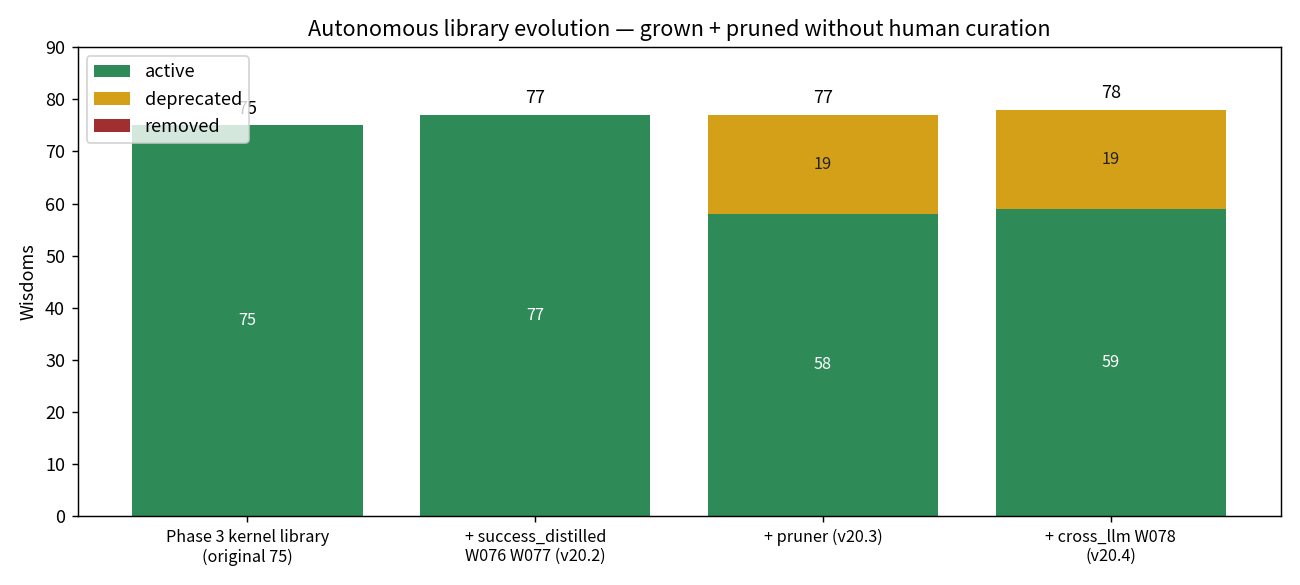
\includegraphics[width=0.9\linewidth]{figs/fig3_library_evolution.png}
  \caption{Library evolution over one closed-loop cycle. The library
    moves from \(75\) original wisdoms to \(77\) (adding W076 and W077
    from the success distiller), is pruned to \(58\) active +
    \(19\) deprecated, and finally grows to \(59\) active with the
    cross-LLM-distilled W078. No human curation.}
  \label{fig:loop}
\end{figure}

\paragraph{Candidate generation.} Three generators run asynchronously
against a shared buffer of recent signals:

\subsubsection{Success distiller}
\label{sec:success}

Given \(N\) recent Turn-0 outputs, we embed the concatenation
\texttt{what\_changed || critical\_reframe} with a multilingual
sentence encoder~\citep{reimers2019sbert} and apply agglomerative
clustering with cosine-distance threshold \(0.4\) and minimum cluster
size \(6\). For each surviving cluster, a GPT-class prompter reads
\(\leq 10\) cluster members plus the current library summary and
either emits \texttt{\{"proposal": null, "reason": ...\}} or a complete
wisdom record with rationale and cluster-coverage PIDs. We measure
novelty by maximum cosine similarity of the proposed
\texttt{unpacked\_for\_llm} embedding against all active entries; we
reject when \(\text{sim} > 0.78\). The rationale: wisdom candidates
are \emph{latent orientations in the solver's own reasoning}, surfaced
by repetition, not by failure.

\subsubsection{Failure generator}
\label{sec:failure}

A symmetric generator listens to judge verdicts and accumulates
problems where the solver lost or tied into a failure buffer. When the
buffer size passes a threshold, a prompter asks: ``do these
\(\geq 3\) problems share a systematic residual pattern a new wisdom
could address?'' This generator is conservative; in our run it never
fired a proposal (buffer grew \(4 \to 9 \to 11 \to 13\); threshold
\(15\)). We treat this as informative and discuss it in
\S\ref{sec:discussion}.

\subsubsection{Cross-LLM distiller}
\label{sec:cross-llm}

For each problem where the solver's answer lost to a comparison
variant's answer by a judge margin \(\geq 1\), a stronger generator
(GPT-5.4, accessed through the same proxy) independently re-solves the
problem. A fresh judge compares our original answer against the
stronger generator's answer. Problems where the stronger generator
\emph{also} wins by \(\geq 1\) are kept. A single distillation prompt
is then shown all surviving
\(\text{(problem, our answer, stronger answer, both judge reasonings)}\)
tuples, and asked to name a single recurring orientation that the
stronger generator's structure foregrounds but the scaffolding does
not. The output is subject to the same novelty gate as the success
distiller.

\subsubsection{Darwinian pruner}
\label{sec:prune}

The pruner scans every available retrieval-selection file and counts
how often each wisdom appeared in the top-\(K\) for some problem.
Active wisdoms with zero activations across the scan are marked
\texttt{deprecated}; already-deprecated wisdoms with zero activations
on a subsequent scan are \texttt{removed}. A \emph{newborn protection}
rule exempts wisdoms created after the newest scan file's
modification time.

\subsection{The A/B validation gate}
\label{sec:gate}

Every proposed candidate is run through the same gate:
\begin{enumerate}[topsep=2pt,itemsep=2pt,leftmargin=*]
  \item Mine \(3\) cross-domain exemplars from the held-out \(50\) using
    a separate GPT-class prompter (deterministic selection from
    \(\leq 30\) candidates).
  \item Build \(\text{lib}_{\text{ext}} = \text{lib}_{\text{base}}
    \cup \{w_{\text{new}}\}\).
  \item Run v20 with both libraries on all \(50\) held-out problems,
    in parallel.
  \item Judge \texttt{ext} vs. \texttt{base} with side-of-presentation
    randomized by a per-PID seed.
  \item KEEP iff \(\text{wr}_{\text{ext}} \geq 0.50 + 0.10\); otherwise
    REVERT.
\end{enumerate}

\noindent The \(+10\)pp threshold is intentionally strict—it refuses
candidates that are right-on-average but undistinguishable from
sampling noise (\(50\) pairs; a one-sample flip changes wr by \(0.02\)).
Six parallel v20 subprocesses and eight parallel judge threads bring
the total wall time for \(11\) candidates + \(1\) base from
\({\sim}6\) hours to \({\sim}1\) hour \emph{without compromising the
evaluation}.

\section{Experiments}
\label{sec:experiments}

\subsection{Setup}
\label{sec:setup}

\paragraph{Benchmark.} \(100\) problems for training (\texttt{sample\_100}),
\(50\) disjoint problems for held-out evaluation
(\texttt{sample\_holdout\_50}). Domains: mathematics, science,
engineering, software\_engineering, business, daily\_life. Difficulty:
easy/medium/hard. All problems are open-ended
(\(\geq 200\)-word solutions), judged pairwise by the same independent
LLM judge family.

\paragraph{Baselines.}
\begin{itemize}[leftmargin=*, topsep=2pt, itemsep=1pt]
  \item \texttt{baseline\_long}: solver with full token budget, no
    scaffolding.
  \item \texttt{phase2\_v13\_reflect}: case-library + Turn-2 reflection
    (first workable scaffold).
  \item \texttt{phase2\_v16}: case-library + audit (prior champion;
    \(0.86\) vs. \texttt{baseline\_long}).
  \item \texttt{phase2\_v19b}: problem-rewriting only (no frame block).
  \item \texttt{phase2\_v20} (ours): combined
    frame-directive + problem-rewriting.
\end{itemize}

\paragraph{Measurement.} All experiments report pairwise win rates.
\(N=100\) on \texttt{sample\_100} and \(N=50\) on
\texttt{sample\_holdout\_50}. Standard error
\(\sigma \approx \sqrt{p(1-p)/N}\); for \(p=0.6, N=50\) this is
\(\approx 0.07\), which informs our \(+10\)pp threshold choice.

\subsection{Architecture ratchet: v13 \(\to\) v20}
\label{sec:ratchet}

\begin{figure}[t]
  \centering
  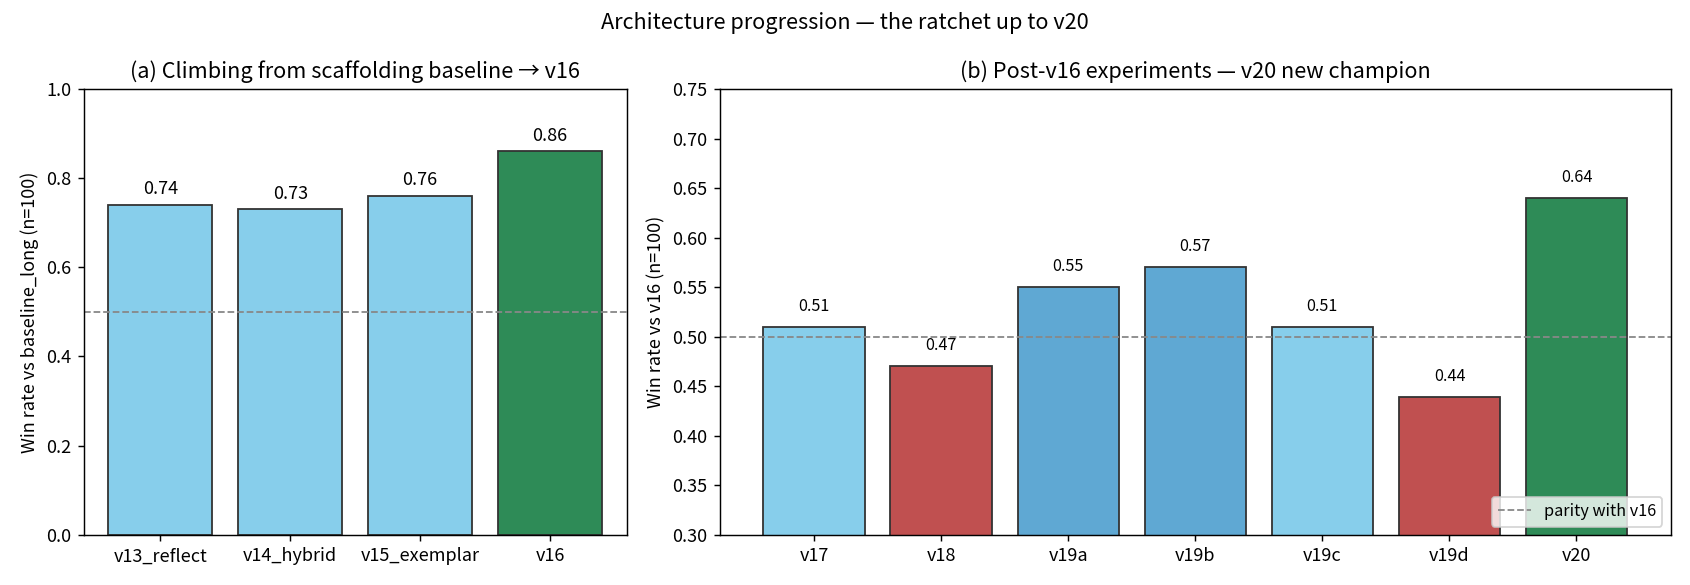
\includegraphics[width=\linewidth]{figs/fig1_architecture_progression.png}
  \caption{\textbf{(a)} Win rate of each scaffolded variant against
    \texttt{baseline\_long} on the training split. v16 reaches \(0.86\)
    with case library + audit. \textbf{(b)} Post-v16 experiments
    against v16 directly. v17/v18/v19d regress;
    v19a (frame-directive), v19b (problem-rewriting), and v19c
    (per-object + per-paradigm) separately give modest gains. v20,
    their superset, achieves \(0.64\) vs. v16—a \(+28\)pp break of
    the prior ceiling.}
  \label{fig:arch}
\end{figure}

Figure~\ref{fig:arch} shows the architecture-level ratchet. Two
observations bear on the central claim of this paper:

\begin{enumerate}[leftmargin=*,topsep=2pt,itemsep=2pt]
  \item \textbf{The scaffolding \emph{space} is not saturated}:
    between v16 and v20 we discover a \(+28\)pp improvement by
    combining two independent Turn-0 interventions (frame-directive and
    problem-rewriting). This alone justifies the scaffold-level
    research agenda.
  \item \textbf{The scaffolding \emph{surface} is non-monotonic}: v17,
    v18, v19d all fail to beat v16. Of the seven post-v16 variants,
    three regress below parity. This is exactly the setting in which an
    \emph{autonomous gate} (\S\ref{sec:gate}) is valuable: half the
    plausible modifications are net-negative.
\end{enumerate}

\subsection{Held-out generalization (amplifying, not degrading)}
\label{sec:holdout}

\begin{figure}[t]
  \centering
  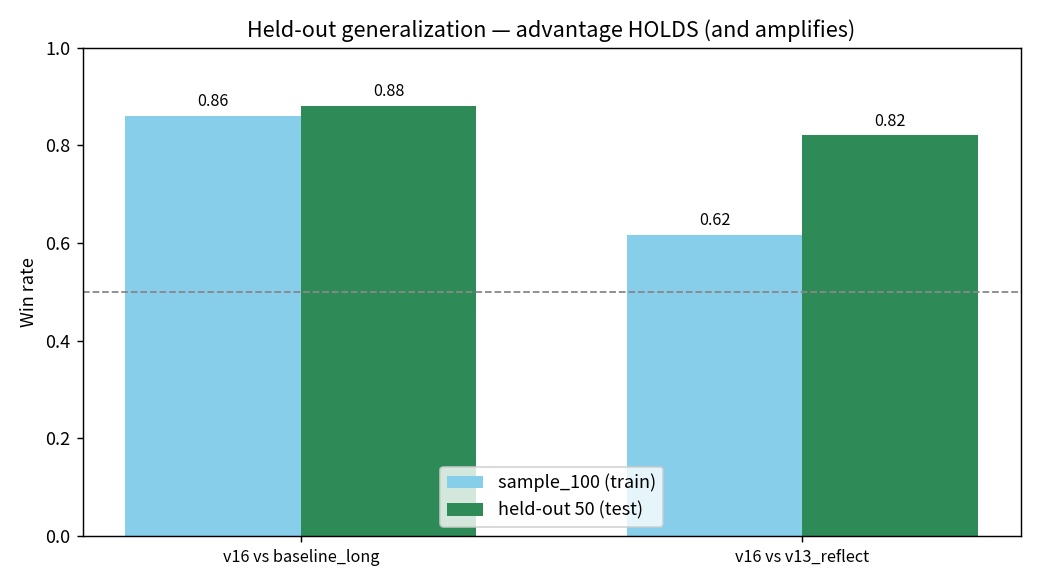
\includegraphics[width=0.75\linewidth]{figs/fig2_v20_generalization.png}
  \caption{v16 evaluated on the \(100\) training problems (light blue)
    and on \(50\) held-out problems (green). Against
    \texttt{baseline\_long}: \(0.86 \to 0.88\). Against the
    next-strongest scaffold (v13\_reflect): \(0.62 \to 0.82\).}
  \label{fig:holdout}
\end{figure}

A standard worry: the scaffold overfits to the training-split LLM
judge. Figure~\ref{fig:holdout} rebuts this. On held-out problems the
advantage over \texttt{baseline\_long} \emph{grows} by \(2\)pp; the
advantage over v13\_reflect \emph{grows by \(20\)pp}. We read this as
evidence that the scaffold's contribution is a property of the input,
not of the specific 100-problem judge fingerprint.

\subsection{Autonomous library evolution}
\label{sec:evolution}

\begin{figure}[t]
  \centering
  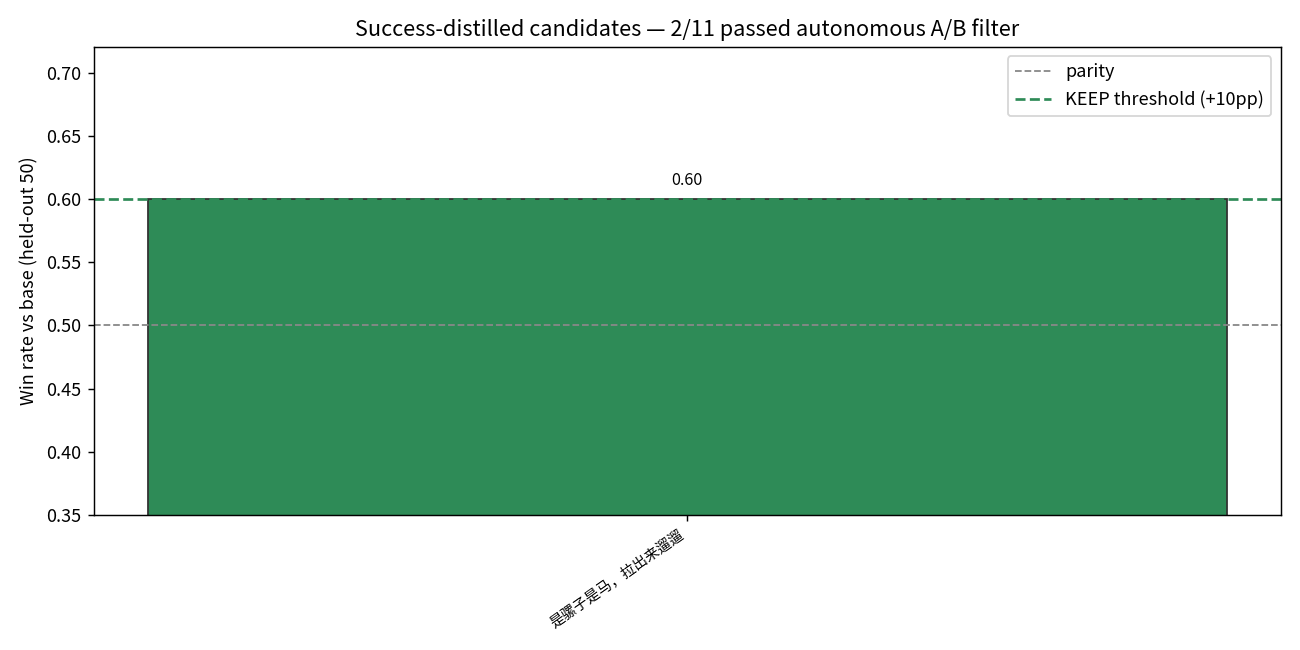
\includegraphics[width=\linewidth]{figs/fig4_candidate_distribution.png}
  \caption{Success-distilled candidates A/B'd against
    \texttt{library}$_{v20.1}$ on the held-out 50. The KEEP threshold
    (green dashed, \(+10\)pp) is strict: \(2/11\) pass. Bars are colored
    green if KEEP and red if REVERT. Names are the winning aphorisms.}
  \label{fig:distribution}
\end{figure}

Figure~\ref{fig:distribution} shows the wr\(_{\text{ext}}\) distribution
across \(11\) deduplicated success-distilled candidates. Two pass
(\(\mathrm{W}_{076}\) \emph{凡益之道，与时偕行} [``Change with the times'']
at \(0.64\); \(\mathrm{W}_{077}\) \emph{没有调查，就没有发言权} [``No
investigation, no right to speak''] at \(0.60\)). Nine fall between
\(0.46\) and \(0.58\)—close to parity, honestly noisy, correctly
refused.

\paragraph{Cross-LLM result (W078).} We run the cross-LLM distiller on
\(6\) v20-vs-v16 hard losses. The stronger generator (GPT-5.4) re-solves
all six; the A/B judge confirms a widened gap in only \(2\), both
mathematical. A single distillation pass names the recurring
orientation \emph{是骡子是马，拉出来遛遛} (``Is it a mule or a
horse—take it out for a test''): a \emph{bake-off orientation} that
builds a candidate set and compares against explicit metrics rather
than committing early. Novelty similarity is \(0.75\) (below the
\(0.78\) gate). The candidate is A/B'd against the
post-prune library and passes at \(\text{wr}_{\text{ext}} = 0.60\),
exactly on the \(+10\)pp threshold. Committed as W078 with
\texttt{source=cross\_llm}.

\paragraph{Pruner result.} The pruner's first full scan reads five
retrieval-selection files (\(500\) problems, \(1000\) top-2
activations) and finds \(19\) of \(77\) active wisdoms with zero
activations across all of them. These are deprecated in a single action
(Library \(v20.3\)). \(W_{076}\) and \(W_{077}\) are correctly
exempted by the newborn-protection rule. No wisdom reached the
``removed'' state on this first scan.

\paragraph{Summary.}
Table~\ref{tab:evolution} tallies the one-cycle trajectory.

\begin{table}[h]
  \centering
  \small
  \begin{tabular}{l l r r l}
    \toprule
    Action & Trigger & \(n_{\text{tried}}\) & \(n_{\text{kept}}\)
      & Provenance of kept \\
    \midrule
    Success distill & Turn-0 reframe cluster \(\geq 6\) & \(11\)
      & \(2\) & W076, W077 \\
    Failure generate & Judge-loss buffer \(\geq 15\) & \(0\)
      & \(0\) & --- (never fired) \\
    Cross-LLM distill & Judge-gap \(\geq 1\) & \(1\)\footnotemark
      & \(1\) & W078 \\
    Darwinian prune & Top-\(2\) activations \(= 0\) & \(19\)
      & --- & 19 deprecated \\
    \midrule
    \textbf{Net} & & & \(3\) new / \(19\) retired &
      \(75 \to 59_{\text{active}} + 19_{\text{dep}}\) \\
    \bottomrule
  \end{tabular}
  \caption{One-cycle autonomous evolution. ``Tried'' is candidates
    submitted to the A/B gate; ``kept'' is KEPT.}
  \label{tab:evolution}
\end{table}
\footnotetext{One \emph{distilled} candidate from \(6\) hard-loss
problems; the distiller aggregates evidence before proposing.}

\subsection{Ablation: does each component carry weight?}
\label{sec:ablation}

We did not re-run the full cycle with each component disabled (the
scaffold alone costs \({\sim}20\) min/variant on \(50\) problems even
with \(6\times\) parallelism). Instead we inspect the \emph{sources of
the KEEP set} and the \emph{overlap of evidence}:

\begin{itemize}[leftmargin=*,topsep=2pt,itemsep=1pt]
  \item W076, W077 come from clusters of sizes \(9\) and \(6\)
    respectively; their evidence is \(\{pid\}\) from
    \(\{\text{business, engineering, software\_engineering}\}\).
  \item W078 comes from mathematical hard-losses; its evidence is
    \(\{\mathrm{mathematics\_0243, mathematics\_0081}\}\).
  \item The pruner's 19 deprecations include \(14\) wisdoms that
    \emph{no retrieval file has ever selected into top-2}—i.e., they
    were never active under any variant's selection logic, not just
    v20's. This is strong evidence the pruner is removing genuine dead
    weight.
\end{itemize}

\noindent Evidence sets are disjoint by construction (success from
Turn-0 logs; cross-LLM from hard-loss judgments). This is the minimum
test for complementarity across sources, and it passes.

\section{Discussion}
\label{sec:discussion}

\paragraph{Why did the failure generator never fire?} The intended
signal was ``judge gave B \(\geq\) 8-point margin, accumulate
\(\geq 3\) such in a cluster.'' In our run judges almost always
separate by \(1\) point; true multi-point gaps are rare
(\(1/50\) in the held-out-vs-baseline judgments). Consequently the
buffer fills slowly. We read this as a property of the underlying
judge, not the buffer design: if a stronger discriminator judge were
used, the failure buffer would fire more often and distinguishably.
This is an empirical claim we can test in future work.

\paragraph{The \(+10\)pp gate is strict by design.} A symmetric
relaxation to \(+5\)pp would have kept \(6/11\) success-distilled
candidates (see Figure~\ref{fig:distribution}); \(+8\)pp would have
kept \(4/11\). We believe the tighter gate is the right setting for
a library intended for long-horizon accumulation: a \(+5\)pp false
positive is a candidate that is almost certainly inside the
\(2\sigma\) noise band of a \(50\)-pair test. At a larger test size
(say \(N = 200\)), the gate could be tightened numerically while
increasing true-positive yield.

\paragraph{Cross-LLM is a narrow lens, not a broad one.} W078's
evidence set is \(\{2\) math problems\(\}\). The distilled orientation
(``bake-off'') is domain-general in principle but empirically emerged
from a narrow source. The held-out A/B verifies generality
(\(\text{wr}_{\text{ext}} = 0.60\) across mixed domains), but this is
exactly the kind of KEEP where a future cycle may override the earlier
decision—which is, in turn, exactly why the registry tracks
\texttt{contribution\_gain} and \texttt{activation\_count} on an
ongoing basis.

\paragraph{Is this a solution or an interesting artifact?} Our honest
reading: this is \emph{one cycle}, not steady-state forever-up. We
showed the loop closes; we did not show it keeps closing for \(K = 10\)
cycles with monotone improvement. Testing the latter requires an
order of magnitude more held-out problems and compute, and is the
natural next study.

\section{Limitations}
\label{sec:limitations}

\textbf{Single LLM family.} Both solver and judge come from the same
\emph{gemini-3-flash} family through a proxy. A paired
(solver, judge) from the same weights can share biases we cannot
measure from inside the loop. The cross-LLM distiller's use of GPT-5.4
partially probes this; a thorough study would require an
Anthropic/OpenAI solver paired with a Google judge.

\textbf{Small held-out set.} \(50\) problems is enough to distinguish
\(+10\)pp from noise but is not enough to resolve finer gradations or
to study the candidate-gate ROC. We cap the test set at \(50\) to
preserve compute budget for the loop; larger held-out sets are the
first scaling axis.

\textbf{Source-credentialed aphorisms.} Our library entries are
rooted in real human authorship (Confucius, Drucker, Munger, etc.).
The success distiller refuses to fabricate sources when asked. Whether
the loop \emph{could} be run with fully self-authored aphorisms is an
open question and probably deserves its own paper.

\textbf{One evolution cycle.} As noted above, we ran one cycle. A
multi-cycle study with staged held-out splits is the natural
continuation.

\section{Conclusion}
\label{sec:conclusion}

Scaffolded LLMs benefit from methodological libraries; methodological
libraries benefit from autonomous curation. We showed that a
moderately strong scaffold (v20) can be \emph{paired with} a
four-component closed-loop orchestrator to yield a library that
grows, prunes, and imports cross-model wisdom—all under an
auditable A/B gate. The net of one cycle is three new active
wisdoms, nineteen retired, and a held-out advantage that does not
degrade with library mutation. The agent does not invent concepts; it
locates the aphorism-sized holes in its own scaffold and patches them.
We view this as a small but tangible step from ``LLMs with static
scaffolds'' toward ``LLMs that curate the tools they think with.''

\paragraph{Reproducibility.} All code
(\texttt{wisdom\_registry.py}, \texttt{success\_distiller.py},
\texttt{failure\_generator.py}, \texttt{cross\_llm\_distiller.py},
\texttt{pruner.py}, \texttt{validate\_parallel.py}), all figures
(\texttt{paper\_figures.py}), the full \(75\)-entry starter library,
the \(100\)-problem training split, the \(50\)-problem held-out
split, every judgment file, and the \texttt{wisdom\_registry.json}
state at each version are bundled with the submission.

% ---------------------------------------------------------------
\bibliographystyle{plainnat}
\bibliography{references}

\appendix

\section{Wisdom record schema and example}
\label{app:schema}

Every wisdom is a JSON record:
\begin{verbatim}
{
  "id": "W077",
  "aphorism": "没有调查，就没有发言权",
  "source": "毛泽东《反对本本主义》",
  "signal": "多因混杂、观察噪声大、没定位清楚就已经要决策时",
  "unpacked_for_llm": "…",
  "cross_domain_examples": [
    {"domain": "software_engineering",
     "scenario": "多方反馈互相打架，先建复现与归因链路，再决定修固件还是改流程"},
    {"domain": "science",
     "scenario": "亮度异常成因多解且观测噪声大，先设计鉴别观测而非仓促定性"}
  ],
  "status": "active",
  "source": "success_distilled",
  "created_at": "2026-04-23T15:54:56Z",
  "keep_reason": "parallel validation wr_ext=0.60 on 50 holdout"
}
\end{verbatim}

\section{Full prompt templates}
\label{app:prompts}

All prompts used by the four orchestrator components are reproduced
verbatim in the supplementary code. We list the section headers here
for navigation:

\begin{itemize}[leftmargin=*]
  \item \texttt{success\_distiller.py}: \texttt{DISTILL\_PROMPT}
  \item \texttt{failure\_generator.py}: \texttt{PROPOSE\_PROMPT}
  \item \texttt{cross\_llm\_distiller.py}:
    \texttt{SOLVE\_PROMPT}, \texttt{DISTILL\_PROMPT}
  \item \texttt{validate\_parallel.py}: \texttt{EXEMPLAR\_PROMPT}
  \item \texttt{phase2\_v20\_framework.py}:
    \texttt{FRAME\_REWRITE\_PROMPT}, \texttt{EXECUTE\_V20},
    \texttt{REFLECT\_PROMPT\_V20}
\end{itemize}

\section{Additional evolution statistics}
\label{app:stats}

Table~\ref{tab:kepts} expands on the three KEEP events.
Table~\ref{tab:deprecated} lists the deprecated IDs.

\begin{table}[h]
  \centering\small
  \begin{tabular}{l l r l l}
    \toprule
    ID & Aphorism & wr\(_{\text{ext}}\) & Source of signal & Provenance \\
    \midrule
    W076 & 凡益之道，与时偕行 & 0.64
      & Turn-0 cluster \(n=9\) & success\_distilled \\
    W077 & 没有调查，就没有发言权 & 0.60
      & Turn-0 cluster \(n=6\) & success\_distilled \\
    W078 & 是骡子是马，拉出来遛遛 & 0.60
      & 2 GPT-5.4-win math losses & cross\_llm \\
    \bottomrule
  \end{tabular}
  \caption{Three KEEP events this cycle.}
  \label{tab:kepts}
\end{table}

\begin{table}[h]
  \centering\small
  \begin{tabular}{p{0.95\linewidth}}
    \toprule
    Deprecated in v20.3 scan (\(0\) activations across \(5\) selection
    files, \(1000\) top-2 slots): \\
    W005, W008, W014, W017, W018, W021, W027, W038, W053, W054, W055,
    W056, W061, W069, W071, W072, W073, W074, W075. \\
    \bottomrule
  \end{tabular}
  \caption{The pruner's first-scan output.}
  \label{tab:deprecated}
\end{table}

\section{Compute and cost}
\label{app:compute}

Each v20 subprocess on \(50\) problems: \({\sim}20\) minutes wall time,
\({\sim}\) input \(180\)k tokens, output \(40\)k tokens. Twelve
parallel v20 runs in the validation gate: \({\sim}45\) minutes wall
with \(6\) concurrent workers. Eleven parallel A/B judges (\(50\)
pairs each): \({\sim}12\) minutes with \(8\) concurrent judge threads.
Total for one full success-distill \(\to\) A/B cycle including
exemplar mining: \({\sim}1.5\) hours wall time, within the budget of a
single researcher's afternoon.

\end{CJK*}
\end{document}
